\chapter{machine learning, statistic, estimations}\label{ml}

EINHEITLICHE VARIABLENBENENUNG!

CTA, much like every other big experiment in (astro-)particle physics,
is going to produce enormous amounts of data.
Depending on the number of installed telescopes, multiple
PB (petabyte per siunitx???) per year are expected to be saved 
on disk and tape \cite{lamanna2015cherenkov}.

Given these enormous amounts of data, it comes as no surprise that
various data reduction techniques need to get applied in 
order to reduce data size.
Multiple machine learning models have proven to be
quite sucessfull in solving classification and
regression problems 
\cite{doi:10.1142/S0218271810017160}
(in TU Netz lesen!).

This thesis focusses on using random forests to
perform gamma/hadron separation, energy estimation(ist das noch drin?)
and source position estimation.
To understand how these algorithms work, I will
give a short introduction into some basics of machine learning.
Because of our focus on random forest algorithms, we will not 
go into unsupervised learning here.

\section{Supervised learning}
In the task of supervised machine learning a model is trained on a
dataset with full information available.
This data can come from monte carlo simulation, but in other contexts 
could also be e.g. historical data.
The trained model can then later be used to estimate values on a dataset, which
lacks the needed information. 

In machine learning we differentiate
the columns(features) of our dataset into a set of \textbf{input} variables $X$ and
a set of \textbf{output} variables $y$. The naming convention for
these sets follows the convention of scikit-learn
\cite{scikit-learn}, \cite{sklearn_api}, a python package for
machine learning algorithm.
We will later use scikit-learn as a basis to implement our machine learning models.
Other terminologies for the two feature sets include
predictors or independent variables for the input, and
responses or dependent variables for the output.

\subsection{Classification}
In (supervised) classification tasks, we want to predict of which of some 
predefined classes the given sample is a member. The possible solutions for $y$
are from a discrete set of values in 
contrast to a regression problem with a continous solution space.
A model that performs classification on data is often referred to as
classifier.

The simplest and most popular case of classification problems
is \textbf{binary classification} \cite{sokolova2009systematic}.
In this case only two distinct
classes exist, which fortunately is all we will need for
our signal/background-separation.
A common example for a classification problem is an e-mail spam filter,
where mails get categorized in at least two categories based
on their content and meta data \cite{DBLP:journals/corr/cs-CL-0006013}.

For binary classification we can define a set of measures
to define the quality of our prediction, starting with the confusion matrix.
These follow the notation and description of
Sokolova and Lapalme \cite{sokolova2009systematic},
with $pos$ referring to the positive (i.e. signal)
and $neg$ referring to the negative (i.e. background) class.

\begin{center}
    \begin{tabular}{ | l | l | l |}
    \hline
    True label & Predicted as $pos$ & Predicted as $neg$ \\
    \hline
    $pos$ & true positive ($tp$) & false negative ($fn$) \\ 
    \hline
    $neg$ & false positive ($fp$) & true negative ($tn$) \\
    \hline
    \end{tabular}
    %\caption{Confusion matrix for a binary classification task with
    %the two labels $pos$ and $neg$.}
    \label{tab:confusion}
\end{center}

An ideal classification would result in
\begin{equation*}
  fp = fn = 0.
\end{equation*}

Based on the confusion matrix, multiple measures 
can be constructed to examine the classifiers performance.
Some of the more common ones include:

\begin{center}
    \begin{tabularx}{\textwidth}{|l|l|X|}
    \hline
    Measure & Formula & Evaluation Focus \\ \hline
    Accuracy & $\frac{tp+tn}{tp+fn+fp+tn}$ & Overall effectiveness of a classifier \\ \hline
    Precision & $\frac{tp}{tp+fp}$ & Class agreement with the positive labels given by the classifier \\
    \hline
    Recall/Sensitivity & $\frac{tp}{tp+fn}$ & Effectiveness of a classifier to identify positive labels \\
    \hline
    F-score & $\frac{(\beta^2+1)tp}{(\beta^2+1)tp+\beta^2fn+fp}$ & Relations between positive labels and predicted labels\\
    \hline
    Specificity & $\frac{tn}{fp+tn}$ & How effectively a classifier identifies negative labels \\ \hline
    AUC & $\frac{1}{2}(\frac{tp}{tp+fn}+\frac{tn}{fp+tn})$ & Classifier’s ability to avoid false classification \\ \hline
    \end{tabularx}
    %\caption{Overview of common metrics for classification tasks based on the 
    %intermediate metrics shown in table \ref{tab:confusion}}
\end{center}

\subsection{Regression}
Regression is the task of predicting a continous variable
from a set of input variables.
The simplest (and historically first) approach 
to this problem is the ordinary linear least squares method.

Given an unrestriced linear model
\begin{align}
	y &= X\beta + e \\
	E(y) &= X\beta \\
	Cov(y) &= \sigma^2 I_n
\end{align}
with a measured vector $y$, the design matrix $X$,
an unknown parameter vector $\beta$, a random error $e$ 
and pairwise orthogonal features $y_i$,
the least-squares solution is given by the solution of 
the minimizing problem in equation \ref{eq:min_least_squares}.

\begin{equation}
	\min_{\beta\in\mathbb{R}^k} \lVert y - X\beta \rVert
	\label{eq:min_least_squares}
\end{equation}

If $(X^TX)^{-1}$ exists, the unique solution for the 
least square estimation of $\beta$ becomes:
\begin{equation}
	\hat{\beta} = (X^TX)^{-1}X^T y.
\end{equation}

The metric, that is minimized by the least-squares solution
is the Mean Squared Error (MSE).
Other metrics for regression tasks include the
Root-Mean-Squared-Error(RMSE)
Mean-Absolute-Error(MAE)
or the Coefficient of Determination ($R^2$).
For complex models, such as neural networks, it is often times 
beneficial to define an own, more fitting measure.

\subsection{Bias and variance}
Bias und Varianz erklären!
-> Motivation für Log Scaling? (Nur wenn wir noch Energie machen?)

\section{Decision trees and random forests}
Methods based on Decision Trees work by recursively partitioning
the parameter space until the output values can easily be estimated
in the respective regions of the parameter space.
Tree-based methods can be applied to both classification and regression tasks.

\subsection{Decision trees, parameter estimation, gini?}
A simple decision tree
for an example classification on the iris dataset
is shown in figure \ref{fig:03_tree}.

\begin{figure}
  \centering
  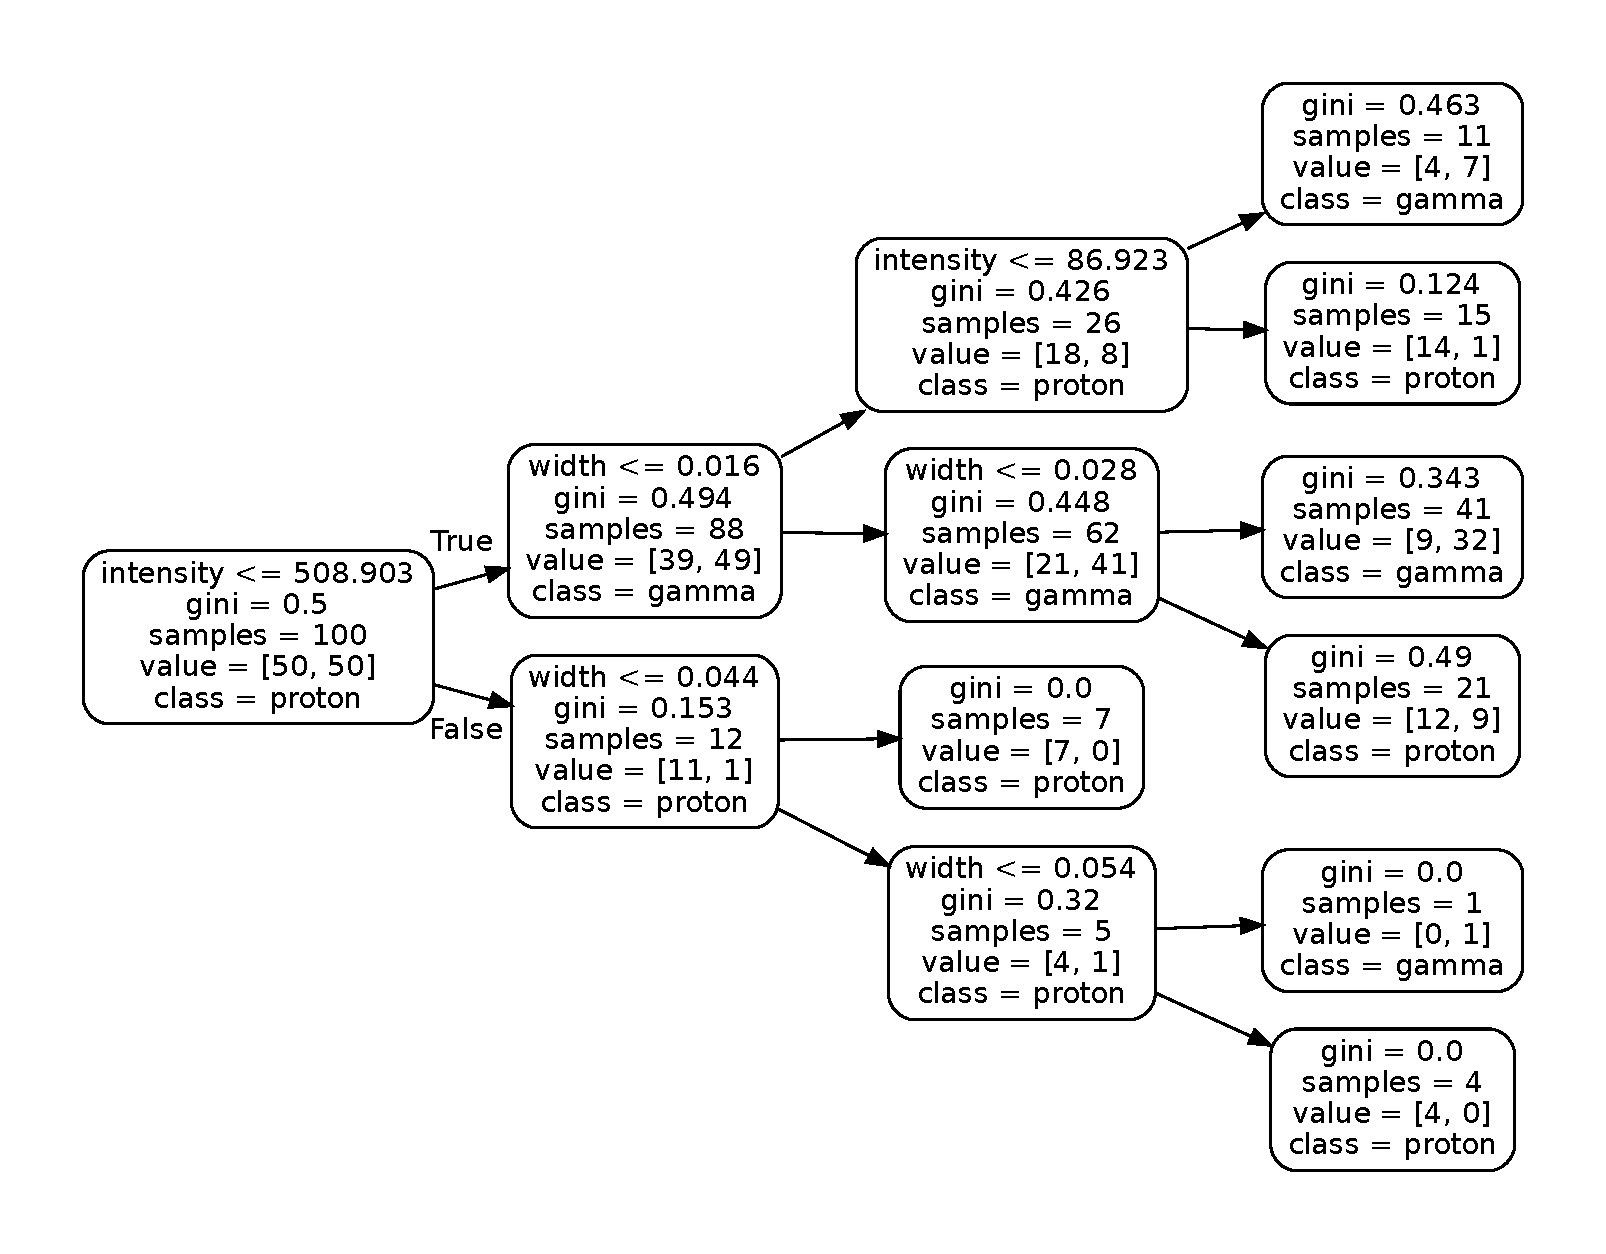
\includegraphics[width=0.7\textwidth]{Plots/decision_tree.pdf}
  \caption{Sample decision tree used to classify flowers in
  the iris dataset \cite{fisher1936use} \cite{sklearn}.}
  \label{fig:03_tree}
\end{figure}

Starting from the root node, a binary split is performed to
split up the data. For each split additional splits are performed
until a stopping criterion is reached.
Choosing the optimal split is defined as minimizing a
pre-defined measure.

For classification tasks often used measures
are the above used gini coefficient (zitat) and the
cross-entropy (zitat).

indizes erklären!
\begin{align}
	\text{Gini coefficient: } &= 1 \\
	\text{Cross-entropy: } &= 2
  \label{eq:03_gini_ce}
\end{align}

A stopping criterion can be defined as the measure reaching a
a defined threshold or not improving anymore.
Alternatively the tree can stop at a predefined depth to 
avoid overly complex models.

For regression tasks sklearn uses the mean squared error 
or mean absolute error and the same principles apply.

While decision trees have the benefit of providing
easily interpretable, low bias models there are some drawbacks to this
approach, namely \cite{hastie2017springer}:
\begin{itemize}
  \item{Instability, high variance}
  \item{Lack of Smoothness}
  \item{Difficulty in Capturing Additive Structure}.
\end{itemize}

Approaches to reducing these problems include
boosting \cite{freund1997decision} and Random Forests \cite{Breiman2001}.

\subsection{Random forests}

Random forests have become one of the standard algorithms
in data analysis tasks, because according to our
experience and \cite{hastie2017springer} they tend to
not overfit (as long as the individual trees have no or little bias)
and generally perform decent without a lot of manual tuning.

The main idea behind random forests is to use multiple, independent
decision trees to suppress the problems single trees have, while
keeping their advantages.
For this to work, the individual trees need not to be correlated.
Consequently the trees cannot all be constructed the same way.
Instead each tree performs splits regarding a random subset of all available variables.
The prediction of the random forest is then the average of
the single trees predictions.
In the case of classification the probabilistic predictions for each class
get averaged.
In other implementations outside of sklearn, the 
the majority vote of the single predictions
is sometimes used (cite something?).

The implementation in sklearn is based on the CART-algorithm by 
Leo Breiman et al (Paper nicht online?).
A single tree performs binary splits $\Theta = (j, t_m)$ 
at each node $m$ in order to split 
the data at this node $Q$ into two subsets 
$Q_\text{left}$
and 
$Q_\text{right}$.
The split consists of a feature $j$ and a threshold $t_m$ and is 
chosen in a way to minimize a given criterion.
Features, that are more important for the task, will
thus appear at the top nodes of the tree.
We will later use the Gini-coefficient and the Mean Squared Error
for the classification and regression tasks respectively.

To make sure the individual trees 
- and their predictions - 
are somewhat independent from each other,
some kind of randomness has to be introduced to the prediction.
In random forests this is for once achieved by giving each tree a 
randomly drawn subsample from the training data.
This is referred to as bootstrapping \cite{efron1992bootstrap}.
Another source of randomness is to perform splits on a node 
based on only a random subsample of the available features.

\iffalse
\section{mean estimation stuff, outlier resistance, unsupervised? clusters?}
warum robuste schätzer?
verwendete algorithmen
\fi
